\section{Durchführung}
\label{sec:Durchführung}

Der Versuchsaufbau ist in Abbildung \ref{fig:aufbau} zu sehen. Zu erkennen ist eine
Quecksilber Dampflampe, deren Licht durch eine Linse zunächst auf eine Spaltblende
gebündelt und nach durchlaufen desselben durch eine weitere Linse auf ein
Geradsichtprisma gebündelt wird. Die Spaltblende gewährleistet, dass nur schmale Linien
des Lichtes am Prisma ankommen, sodass diese durch das Prisma aufgefächert und voneinander getrennt
werden. Die genaue Justierung der dargestellten Elemente ist von großer Bedeutung,
da nur sehr geringe Ströme gemessen werden.

\begin{figure}
  \centering
  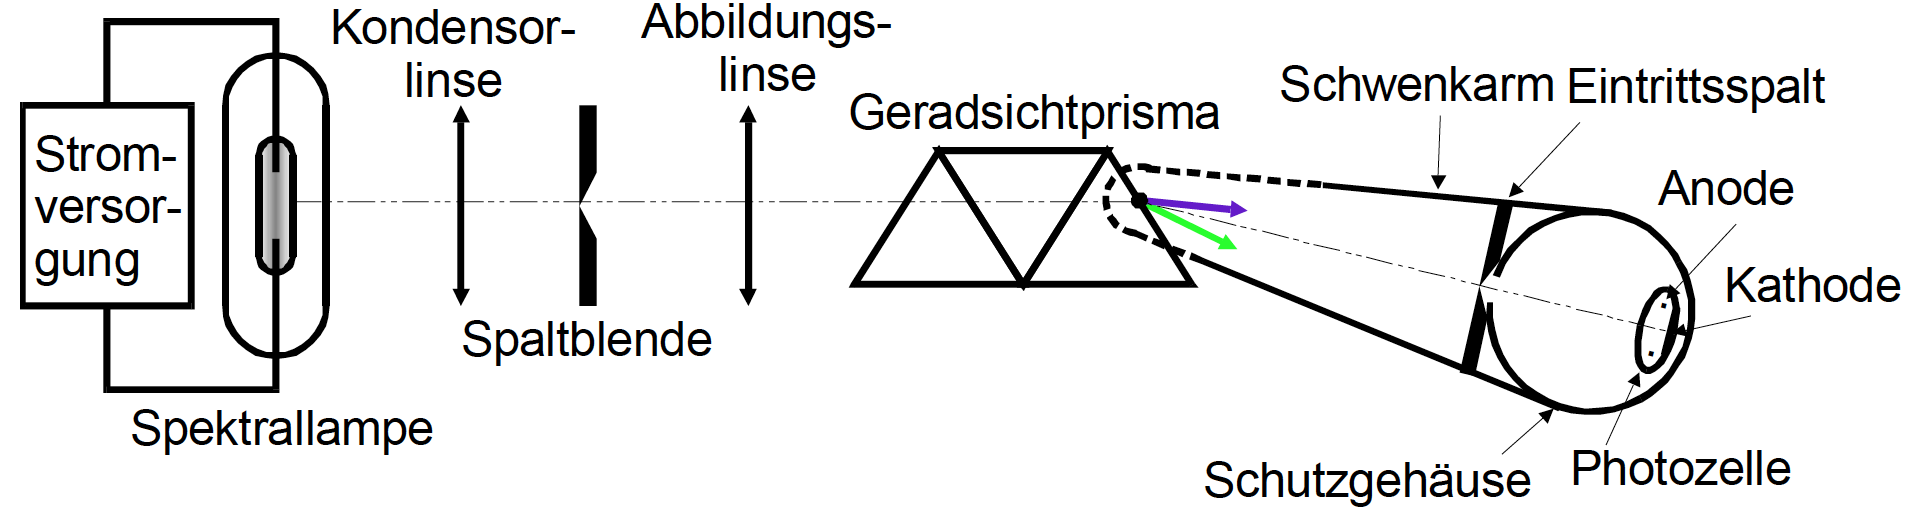
\includegraphics[width=\textwidth]{data/aufbau.png}
  \caption{Skizze des Versuchsaufbaus \cite{Versuchsanleitung}.}
  \label{fig:aufbau}
\end{figure}

Die Photozelle wird nacheinander mit monochromatischem Licht verschiedener Wellenlängen
bestrahlt und es wird jeweils der Phototstrom in Abhängigkeit von der angelegten
Gegenspannung gemessen. Dafür wird eine Gegenspannung eingestellt, bei der der
Phtotstrom verschwindet. Daraufhin wird die Gegenspannung in gleichmäßigen intervallen
reduziert und der zugehörige Photostrom wird gemessen. Es werden dabei die gelbe,
die grüne, die blaugrüne, die beiden violetten und eine ultraviolette Spekrallinie
untersucht.

Außerdem wird für Licht der Wellenlänge $\lambda=578\,$nm der Photostrom für Spannungen
in einem Bereich von $U=-19\,$V bis $U=19\,$V in gleichmäßigen Abständen gemessen.
